\documentclass{report}
\usepackage{graphicx}  % For adding images
\usepackage{xcolor}    % Color support (before hyperref)
\usepackage{hyperref}  % For clickable links
\usepackage{titlesec}  % For customizing titles
\usepackage{fancyhdr}  % For custom headers and footers
\usepackage{lmodern}   % Modern font
\usepackage{etoolbox}  % Required for \preto (if needed)
\usepackage{ragged2e}  % For text justification
\usepackage{setspace}  % For line spacing
\usepackage{subcaption} % Essential for subfigures

\definecolor{darkblue}{RGB}{34, 102, 153}  % Chapter title
\definecolor{mediumblue}{RGB}{50, 120, 180}  % Section title
\definecolor{lightblue}{RGB}{100, 140, 200}  % Subsection title
\definecolor{subblue}{RGB}{120, 160, 220}     % New color for subsubsection
\definecolor{teal}{RGB}{30, 120, 120}  % Résumé & Table of Contents
\definecolor{grayline}{RGB}{180, 180, 180}  % Line under titles

\renewcommand{\normalsize}{\fontsize{13pt}{15pt}\selectfont}  % Default text size
% --- Improving paragraph appearance ---
\AtBeginDocument{
    \justifying          
    \linespread{1.5}      % More readable line spacing
    \spaceskip=0.6em plus 1pt minus 1pt  % Increase word spacing
    \setlength{\parindent}{15pt}  % Indent first line of each paragraph
    \setlength{\parskip}{6pt}  % Add space between paragraphs
}

% --- Personnalisation du style des chapitres ---
\titleformat{\chapter}[block]  
{\centering\bfseries\Huge\vspace{5cm}\color{darkblue}}  % Centre horizontalement, police moderne et grande
{Chapitre \thechapter:}  % Chapitre numéroté sous la forme "Chapitre X: "
{10pt}  
{\parbox{0.9\textwidth}{\centering}} % Wrap inside a centered box
[\vspace{0.4pt}\rule{\textwidth}{1pt}\vspace{10pt}] % Ligne SOUS le titre

%sections styling
\titleformat{\section}
{\Large\bfseries\color{mediumblue}}  % Medium Blue for Sections
{\thesection}{1em}{}

%subsections styling
\titleformat{\subsection}
{\large\bfseries\color{lightblue}}  % Light Blue for Subsections
{\thesubsection}{1em}{}

% Custom subsubsection style
\titleformat{\subsubsection}[block] % Shape
  {\normalfont\bfseries\color{subblue}} % Format
  {\thesubsubsection} % Label
  {0.5em} % Horizontal separation between label and title
  {} % Before-code
  [\vspace{-0.5em}] % After-code (reduces space after header)

\titlespacing*{\subsubsection}{0pt}{1.5\baselineskip}{0.5\baselineskip} % {left}{before}{after}

% --- Force chaque section à commencer sur une nouvelle page ---
\preto\section{\clearpage}

% --- Customizing the TOC title ---
\renewcommand{\contentsname}{\textcolor{teal}{\textbf{Table des Matières}}}
\renewcommand{\listfigurename}{\textcolor{teal}{\textbf{Liste des Figures}}}

% Hyperref settings to remove color, border, and line
\hypersetup{
    colorlinks=false,       % Disable colored links
    linkbordercolor={1 1 1}, % Remove border color (set to white)
    pdfborder={0 0 0},     % Remove the border around links
}

\title{Rapport du Projet de Fin d'Études}
\author{Fatim Ezzahrae Akniz \\ Fatima Ezzahra Benzeroual}

\begin{document}

\maketitle


\vspace*{\fill} % Vertical centering

\section*{\textcolor{teal}{Résumé}}  % Unnumbered section in teal
\justifying
Ce projet scolaire consiste en une plateforme web permettant aux utilisateurs de créer et personnaliser des CV professionnels, avec la possibilité de les exporter en format PDF ou d'en récupérer le code source LaTeX pour des modifications avancées.  

La plateforme intègre également un espace de publication d'offres d'emploi où les recruteurs peuvent poster des annonces contenant les détails du poste et leurs coordonnées, permettant aux candidats de les contacter directement.  

Dotée d'une architecture rôle-based, l'application offre aux administrateurs un tableau de bord pour gérer les modèles de CV et suivre l'activité globale, tandis que les utilisateurs bénéficient d'une interface intuitive pour créer et gérer leurs CV.  

Développée avec React pour le frontend, Express.js pour le backend et MongoDB comme base de données non relationnelle, cette application a permis d'explorer des défis techniques tels que la compilation de documents LaTeX côté serveur, la gestion des autorisations basée sur les rôles, et la conception d'une API REST sécurisée.  

Ce projet illustre comment les technologies web modernes peuvent répondre à des besoins concrets tout en offrant une expérience utilisateur fluide et professionnelle.  

\vspace*{\fill} % Vertical centering

{ % Open a temporary scope
\titleformat{\chapter}{\normalfont\Huge}{}{0pt}{}  % Reset style
\tableofcontents
\listoffigures  % List of Figures
} % Close the scope
\clearpage

\chapter{Introduction}
\clearpage
\justifying

\vspace*{\fill} % Vertical centering
Ce projet consiste en une plateforme web permettant aux utilisateurs de générer des CV professionnels au format LaTeX, avec la possibilité de les télécharger en PDF ou d'en récupérer le code source.  

La plateforme intègre également un système de gestion des offres d'emploi et une administration avancée. Les utilisateurs peuvent créer, modifier et partager leurs CV, tandis que les administrateurs ont accès à des statistiques (nombre d’utilisateurs, CV générés, etc.) et peuvent gérer des modèles de CV personnalisables.  

Développée avec une stack React pour le frontend, Express.js pour le backend et MongoDB pour la base de données, cette application suit une architecture rôle-based (utilisateur/admin) et répond à un besoin de personnalisation et d’automatisation dans la création de documents professionnels.  

Ce rapport détaille les choix techniques, les fonctionnalités clés, les défis rencontrés et les pistes d’amélioration. 

\vspace*{\fill} % Vertical centering

\chapter{Présentation de l'organisme}
\section{Ecole Supérieure de Technologie de Safi}
L’Ecole Supérieure de Technologie de Safi (ESTS) fondée en Septembre 1992, établissement phare de l’université Cadi Ayyad, est une institution académique reconnue pour sa formation technique (DUT) et professionnelle (LP) à partir de l’année universitaire 2014-2015.  

Située à Safi, une ville côtière du Maroc, l’ESTS offre une gamme diversifiée de programmes dans les domaines de l’ingénierie, des sciences appliquées, et de la gestion. Depuis sa création, l’ESTS s’est engagé à fournir une éducation moderne et pertinente, en mettant l’accent sur l’excellence académique et l’innovation.  

Dans le but est de préparer ses étudiants à répondre aux défis du marché du travail avec des compétences pratiques et théoriques solides. Supervisé par un corps professoral qualifié et infrastructures modernes, l’ESTS se positionne comme un acteur clé dans le développement de talents capables de contribuer au progrès technologique et économique de la région.  

\chapter{Analyse des besoins}
\section{Besoins fonctionnels}

L’analyse des besoins fonctionnels a permis d’identifier les principales exigences du système, classées selon les différents acteurs (utilisateurs et administrateurs).

\par

\textbf{1. Besoins des Utilisateurs (Candidats)}

\textbf{Gestion des CV :}
\begin{itemize}
    \item Créer, modifier et supprimer un CV à partir de modèles prédéfinis.
    \item Prévisualiser le CV avant exportation.
    \item Exporter le CV au format PDF ou en code LaTeX pour édition ultérieure.
    \item Consulter et gérer l'historique de ses CV.
\end{itemize}

\par

\textbf{Offres d'emploi :}
\begin{itemize}
    \item Consulter la liste des offres disponibles.
    \item Contacter directement le recruteur via les coordonnées fournies.
\end{itemize}

\par

\textbf{2. Besoins des Recruteurs}

\textbf{Publication d'offres :}
\begin{itemize}
    \item Remplir un formulaire structuré (titre, description, compétences requises, coordonnées).
    \item Modifier ou supprimer une offre publiée.
\end{itemize}

\par

\textbf{3. Besoins des Administrateurs}

\textbf{Gestion des modèles de CV :}
\begin{itemize}
    \item Ajouter et supprimer des modèles de CV (fichiers LaTeX prédéfinis).
\end{itemize}

\par

\textbf{Supervision de la plateforme :}
\begin{itemize}
    \item Visualiser les statistiques d'utilisation (nombre d'utilisateurs, CV générés, offres actives).
\end{itemize}

\par

\textbf{4. Fonctionnalités Techniques Requises}

\textbf{Système d'authentification sécurisé :}
\begin{itemize}
    \item Gestion des rôles et permissions (accès différenciés entre utilisateurs et administrateurs).
\end{itemize}

\textbf{Génération dynamique de PDF :}
\begin{itemize}
    \item Compilation LaTeX côté serveur pour générer des CV au format PDF.
\end{itemize}

\textbf{Base de données NoSQL (MongoDB) :}
\begin{itemize}
    \item Stockage des CV, offres et utilisateurs avec des schémas flexibles.
\end{itemize}

\par

Cette analyse a servi de base pour la conception de l'architecture et le développement des différentes briques fonctionnelles du système.

\section{Besoins non-fonctionnels}

Les besoins non fonctionnels définissent les exigences techniques et qualitatives de notre plateforme, garantissant son bon fonctionnement dans des conditions réelles d'utilisation.

\par

Contrairement aux besoins fonctionnels qui décrivent \textbf{ce que le système fait}, ces spécifications déterminent \textbf{comment il le fait}, en termes de performance, sécurité, facilité d'utilisation et maintenabilité.

\par

Cette section présente les critères essentiels que notre application doit respecter pour offrir une expérience fiable et professionnelle à ses utilisateurs. Ces exigences guident nos choix techniques et architecturaux tout au long du développement.

\par

\textbf{1. Performance}
\begin{itemize}
    \item La plateforme doit rester stable avec plusieurs utilisateurs connectés en même temps.
    \item La génération de PDF ne doit pas prendre plus de 10 secondes.
\end{itemize}

\par

\textbf{2. Sécurité}
\begin{itemize}
    \item Protection des comptes par mot de passe sécurisé.
    \item Seul l'auteur peut modifier/supprimer son CV.
    \item Les administrateurs ont un accès spécial pour gérer les templates.
\end{itemize}

\par

\textbf{3. Facilité d'utilisation}
\begin{itemize}
    \item Interface simple et intuitive.
    \item Processus de création de CV en quelques étapes seulement.
    \item Compatible avec les navigateurs modernes.
\end{itemize}

\par

\textbf{4. Maintenance}
\begin{itemize}
    \item Code organisé pour faciliter les modifications futures.
    \item Documentation basique du fonctionnement.
\end{itemize}

\par

\textbf{5. Contraintes techniques}
\begin{itemize}
    \item Doit fonctionner avec les packages LaTeX de base.
    \item Utilisation de MongoDB pour stocker les données.
    \item Déploiement possible sur un serveur standard.
\end{itemize}

\chapter{Conception}
\section{UML}

Pour formaliser l'architecture et les interactions de notre application, nous avons utilisé UML (Unified Modeling Language). Ce langage de modélisation standardisé nous a permis de :

\begin{itemize}
    \item Visualiser clairement la structure du système (classes, composants)
    \item Planifier les fonctionnalités avant l'implémentation
    \item Communiquer efficacement au sein de l'équipe
\end{itemize}

\par

Les diagrammes UML produits incluent :

\begin{itemize}
    \item \textbf{Diagramme de cas d'utilisation} : Interactions entre acteurs (utilisateurs, admin) et fonctionnalités.
    
    \item \textbf{Diagramme de classes} : Structure des données (modèles MongoDB schématisés en "classes").
    
    %\item \textbf{Diagrammes de séquence} : Flux critiques (ex. : génération d'un PDF).
\end{itemize}

\vspace{1cm}

\begin{figure}[h]
    \centering
    
\includegraphics[width=0.8\textwidth]{./imgs/umlLogo.png}
    \caption{UML Logo}
    \label{fig:uml_logo}
\end{figure}

\section{Diagramme des cas d'utilisation}

Le diagramme des cas d'utilisation (Figure~\ref{fig:use_case_diagram}) présente les interactions entre les différents acteurs du système et les fonctionnalités principales. On distingue deux types d'acteurs principaux :

\begin{itemize}
    \item \textbf{Utilisateur standard} : Peut gérer ses CV, consulter les offres d'emploi et contacter les recruteurs
    \item \textbf{Administrateur} : Dispose de droits supplémentaires pour gérer les templates et superviser l'activité globale
\end{itemize}

\begin{figure}[htbp]
    \centering
    \makebox[\textwidth]{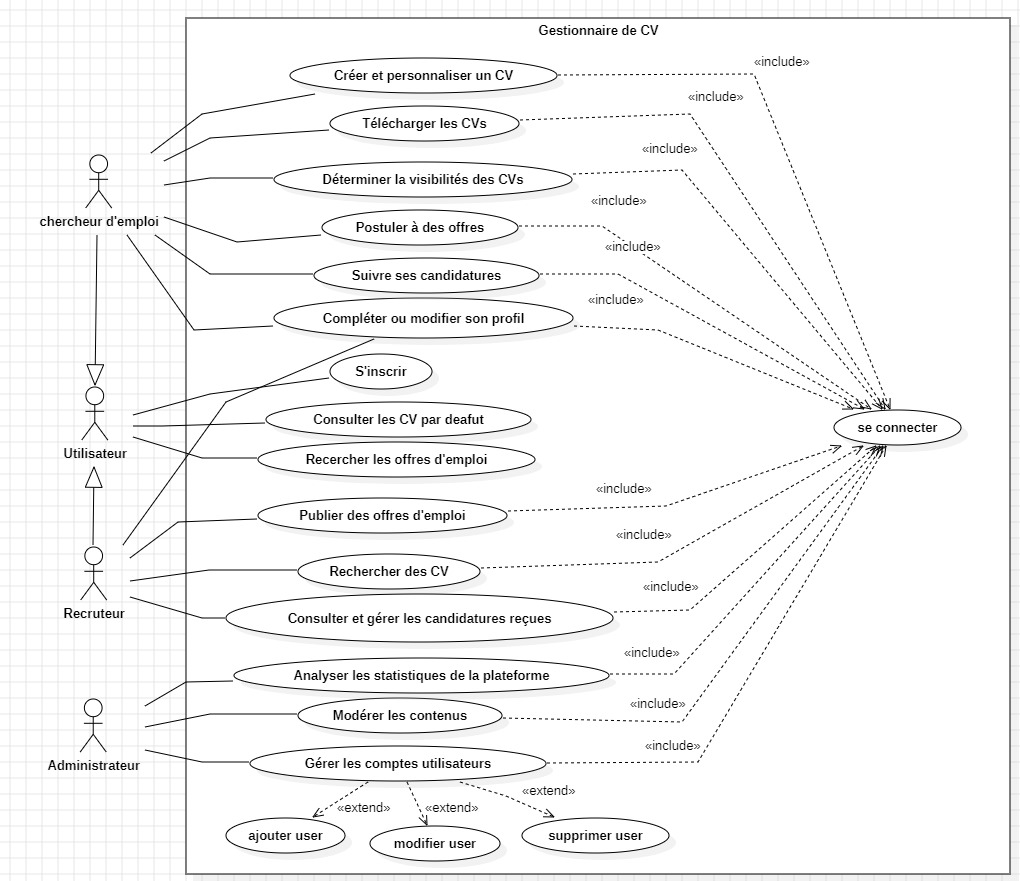
\includegraphics[width=1.5\linewidth]{./imgs/useCaseDiagram.jpg}}
    \caption{Diagramme des cas d'utilisation}
    \label{fig:use_case_diagram}
\end{figure}

\section{Diagramme de classe}

Le diagramme de classes (Figure~\ref{fig:class_diagram}) présente la structure objet du système et les relations entre les différentes entités. Les principales classes représentées sont :

\begin{itemize}
    \item \textbf{User} : Gère l'authentification et les profils des utilisateurs
    \item \textbf{CV} : Contient les informations des curriculum vitae et leurs templates
    \item \textbf{JobOffer} : Stocke les données des offres d'emploi publiées
    \item \textbf{Template} : Modélise les différents modèles de CV disponibles
\end{itemize}

\vspace{2cm}

\begin{figure}[htbp]
    \centering
    \makebox[\textwidth]{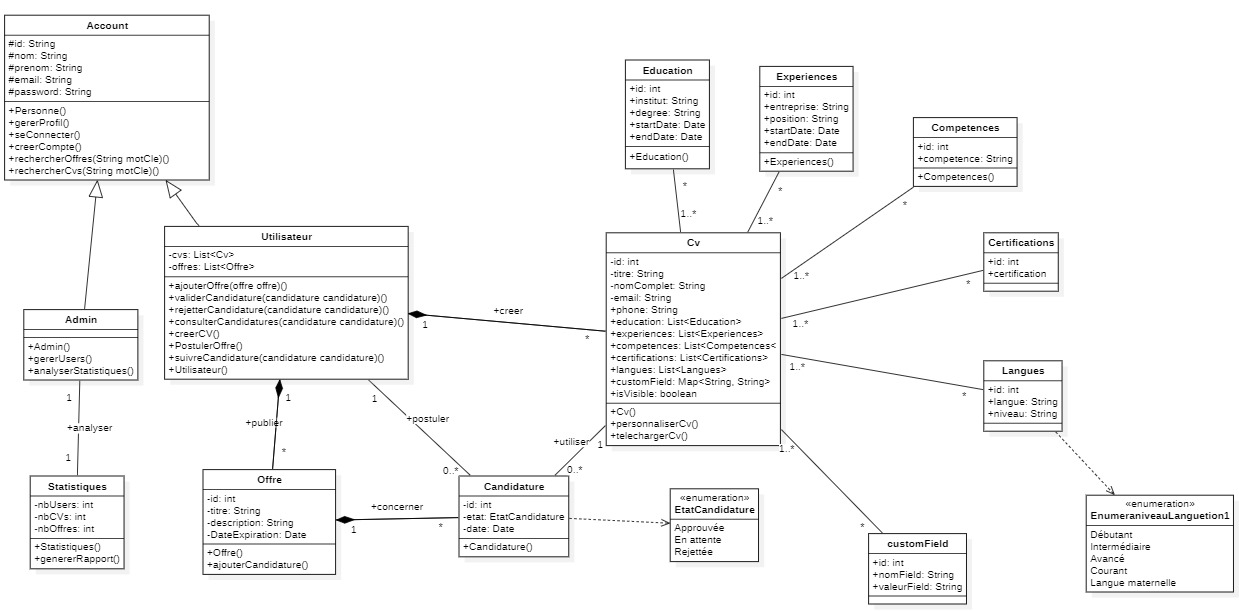
\includegraphics[width=1.6\linewidth, height=0.7\textheight]{./imgs/classDiagram.jpg}}
    \caption{Diagramme de classes}
    \label{fig:class_diagram}
\end{figure}
%\section{Diagrammes de séquence}

\chapter{Outils et Langages utilisés}
\section{Introduction}

Ce chapitre présente l'écosystème technologique choisi pour le développement de notre plateforme de gestion de CV. La sélection des outils s'est basée sur :

\begin{itemize}
    \item Les exigences techniques identifiées dans l'analyse des besoins
    \item La compatibilité entre les différents composants
    \item Les compétences acquises dans le cadre de notre formation
\end{itemize}

Notre solution combine des technologies modernes pour le frontend, le backend et la gestion des données. Ce choix technologique permet une séparation claire des responsabilités tout en garantissant une bonne maintenabilité du projet.
\section{Outils}
\subsection{React}
Framework JavaScript pour interfaces utilisateurs. Choisi pour :
\begin{itemize}
    \item Architecture composants réutilisables
    \item Gestion d'état efficace (hooks, contexte)
    \item Large écosystème de librairies complémentaires
\end{itemize}
\begin{center}
    
\includegraphics[width=0.8\linewidth]{./imgs/reactLogo.jpg}
\end{center}

\subsection{Express.js}
Framework web minimaliste pour Node.js. Sélectionné pour :
\begin{itemize}
    \item Création rapide d'API REST
    \item Middleware modulable
    \item Compatibilité avec les drivers MongoDB
\end{itemize}
\begin{center}
    
\includegraphics[width=0.8\linewidth]{./imgs/expressLogo.jpg}
\end{center}

\subsection{MongoDB}
Base de données NoSQL orientée documents. Adoptée car :
\begin{itemize}
    \item Schéma flexible adapté aux CV personnalisés
    \item Requêtes JSON natives
    \item Scaling horizontal aisé
\end{itemize}
\begin{center}
    
\includegraphics[width=0.6\linewidth]{./imgs/mongodbLogo.jpg}
\end{center}

\subsection{Visual Studio Code}
EDI moderne par Microsoft. Utilisé grâce à :
\begin{itemize}
    \item Support excellent du JavaScript/TypeScript
    \item Extensions LaTeX et UML pertinentes
    \item Débogueur intégré pour le full-stack
\end{itemize}
\begin{center}
    
\includegraphics[width=0.6\linewidth]{./imgs/vscodeLogo.jpg}
\end{center}

\clearpage

\subsection{StarUML}
Logiciel de modélisation UML. Choisi pour :
\begin{itemize}
    \item Génération automatique de diagrammes
    \item Export PNG/PDF de qualité
    \item Gratuit pour les projets académiques
\end{itemize}
\begin{center}
    
\includegraphics[width=0.9\linewidth]{./imgs/starumlLogo.jpg}
\end{center}


\chapter{Implémentation du Projet}
\section{Introduction}

Cette documentation visuelle présente l'application opérationnelle à travers ses interfaces principales : création de CV (export PDF/LaTeX), publication d'offres d'emploi, et gestion administrative des templates et utilisateurs. Les captures d'écran illustrent le flux complet des fonctionnalités implémentées.

\section{Application web}

\subsection{Pages publiques}  % New subsection
\subsubsection{Page d'accueil}
\begin{figure}[h]
    \centering
    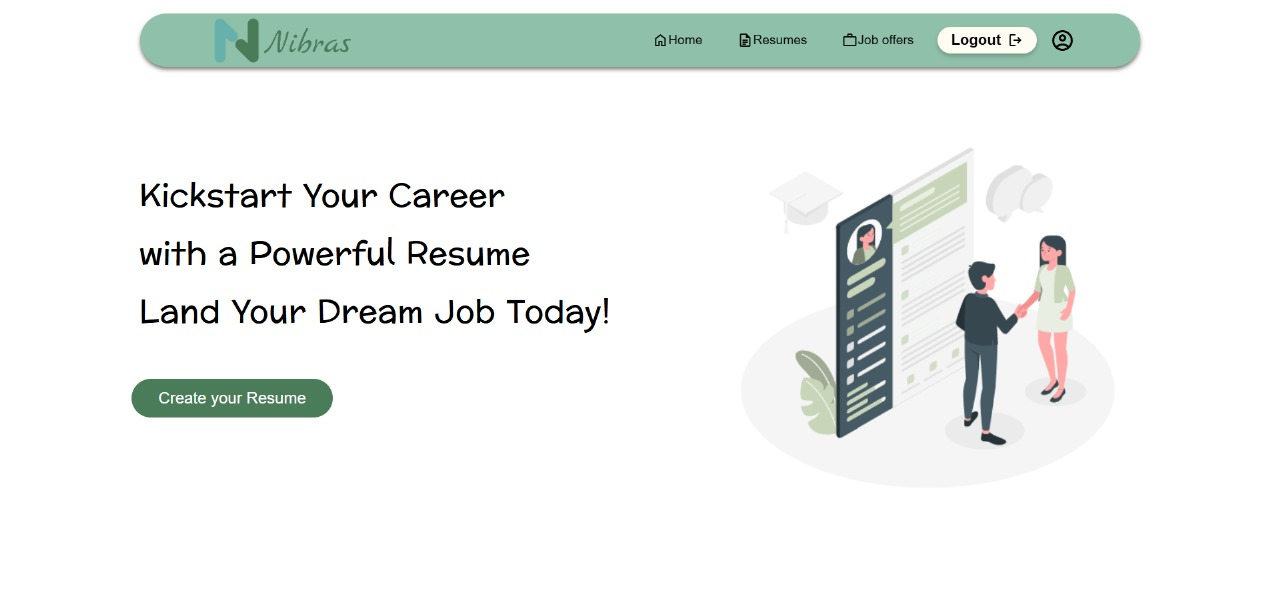
\includegraphics[width=1.4\linewidth]{./imgs/screens/home.jpg}
    \caption{Page d'accueil}
\end{figure}

\clearpage

\subsubsection{Authentification}
\begin{figure}[h]
    \centering
    \begin{subfigure}{0.45\textwidth}
        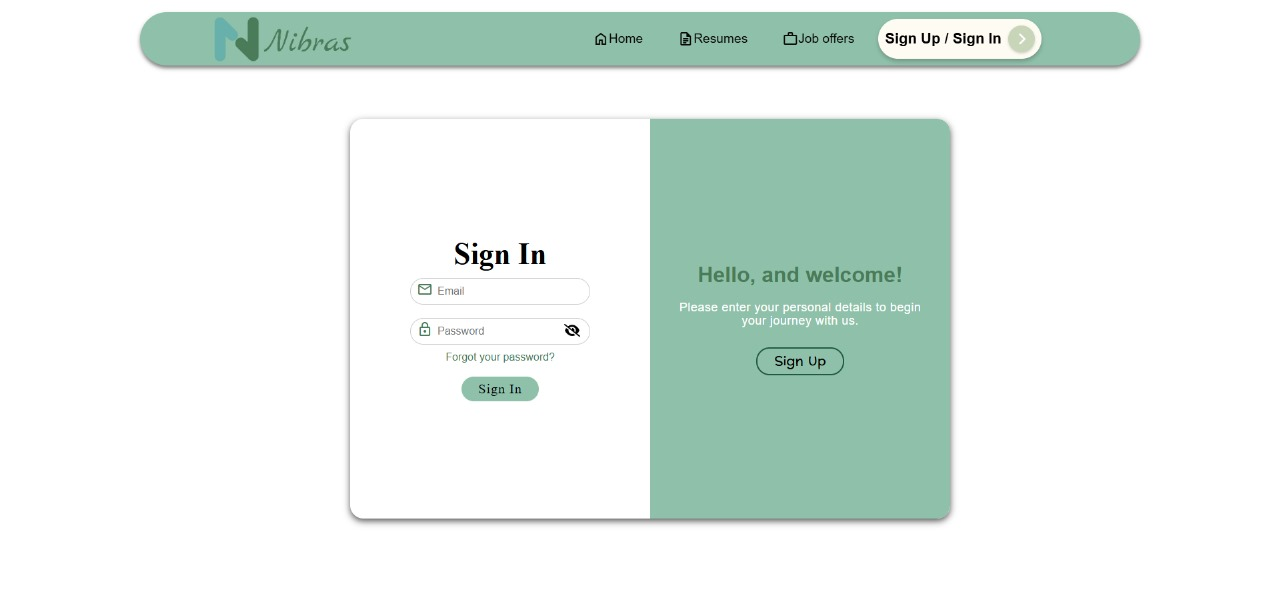
\includegraphics[width=\linewidth]{./imgs/screens/login.jpg}
        \caption{Page de connexion}
    \end{subfigure}
    \hfill
    \begin{subfigure}{0.45\textwidth}
        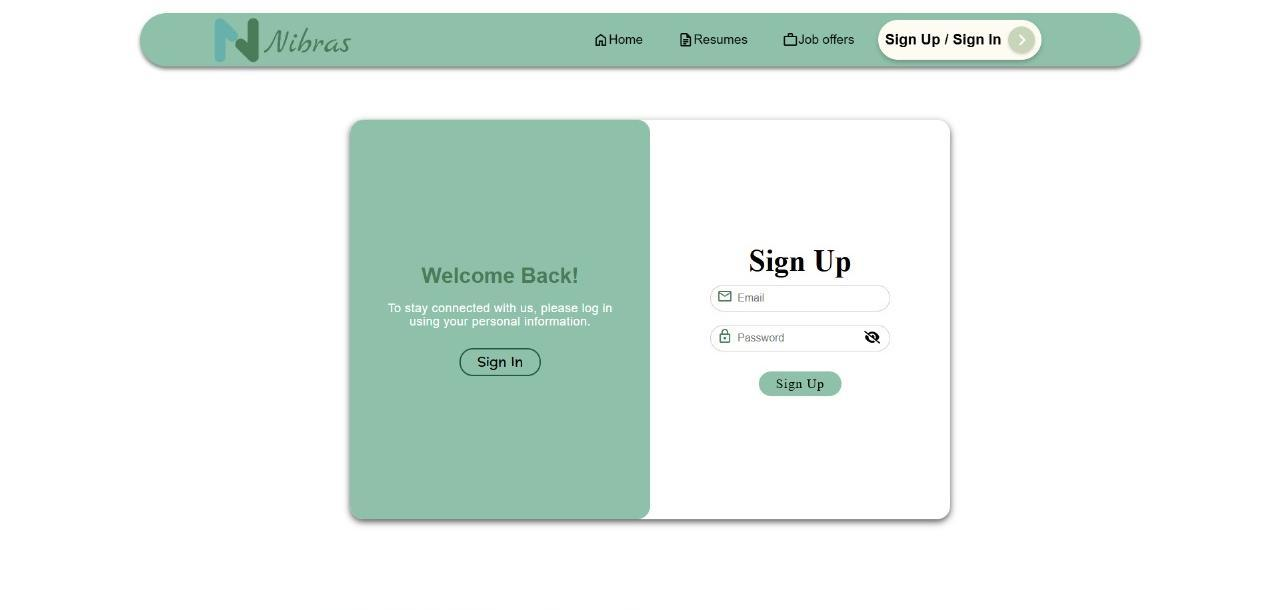
\includegraphics[width=\linewidth]{./imgs/screens/signUP.jpg}
        \caption{Page d'inscription}
    \end{subfigure}
    \caption{Interface d'authentification}
\end{figure}

\subsection{Interface utilisateur}

\subsubsection{Creation de CV}
\begin{figure}[h]
    \centering
    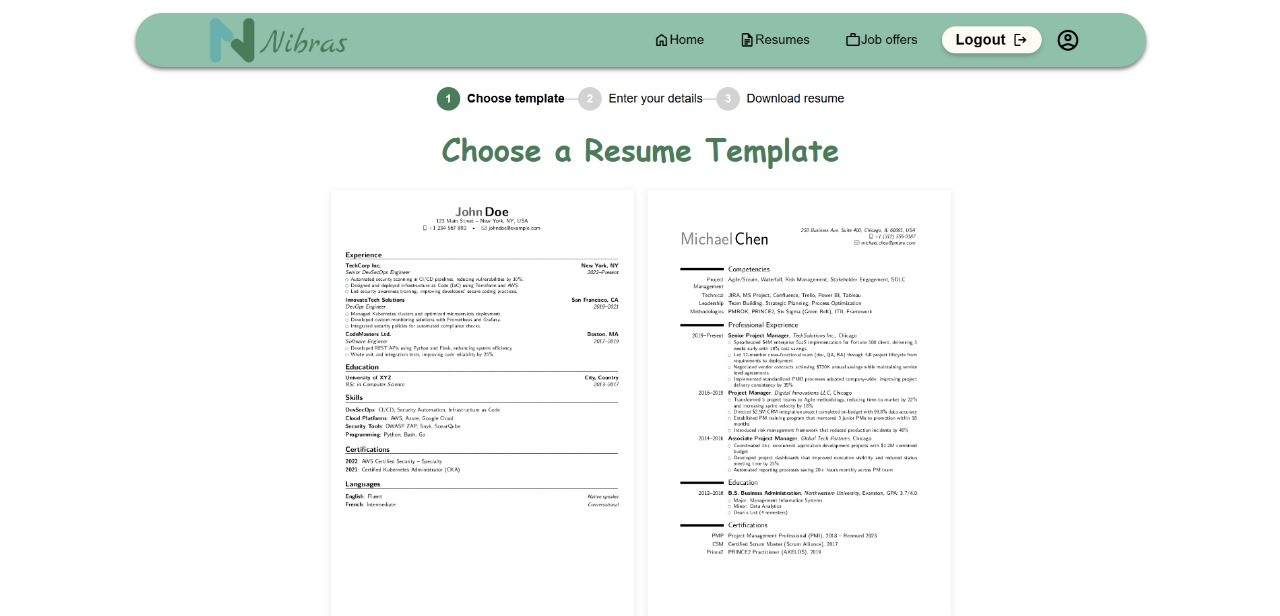
\includegraphics[width=1.2\linewidth]{./imgs/screens/tempListe.jpg}
    \caption{Liste des templates disponibles}
\end{figure} 

\begin{figure}[h]
    \centering
    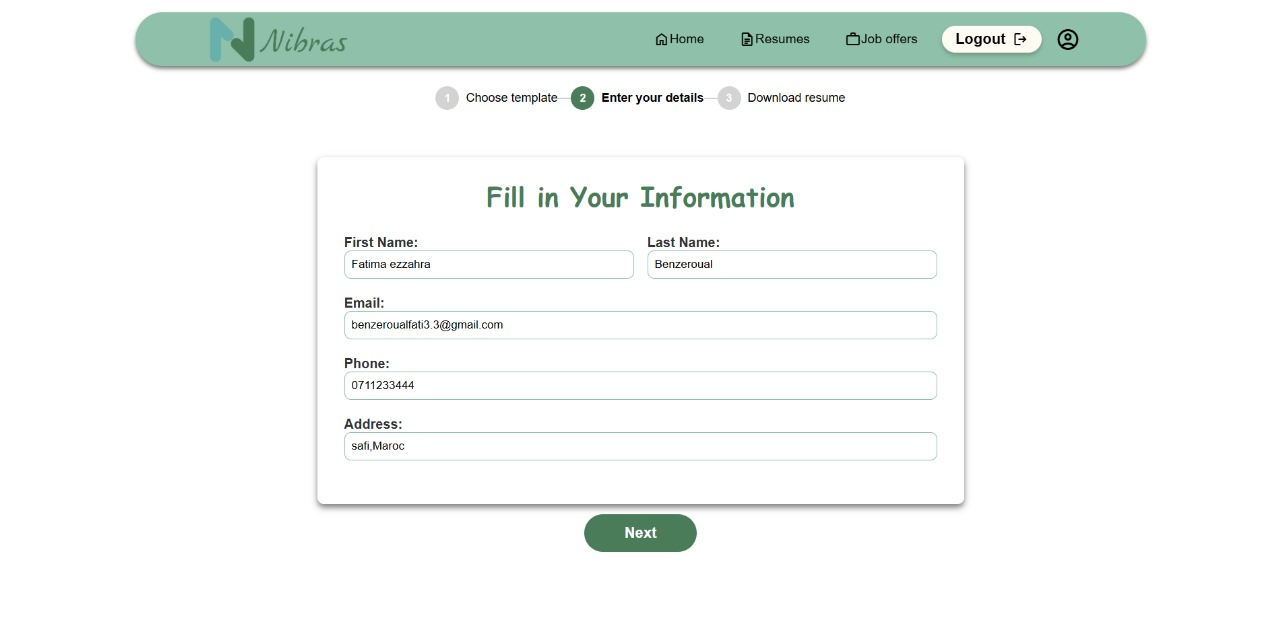
\includegraphics[width=1.2\linewidth]{./imgs/screens/personalForm.jpg}
    \caption{Formulaire pour les informations personnelles}
\end{figure} 

\begin{figure}[h]
    \centering
    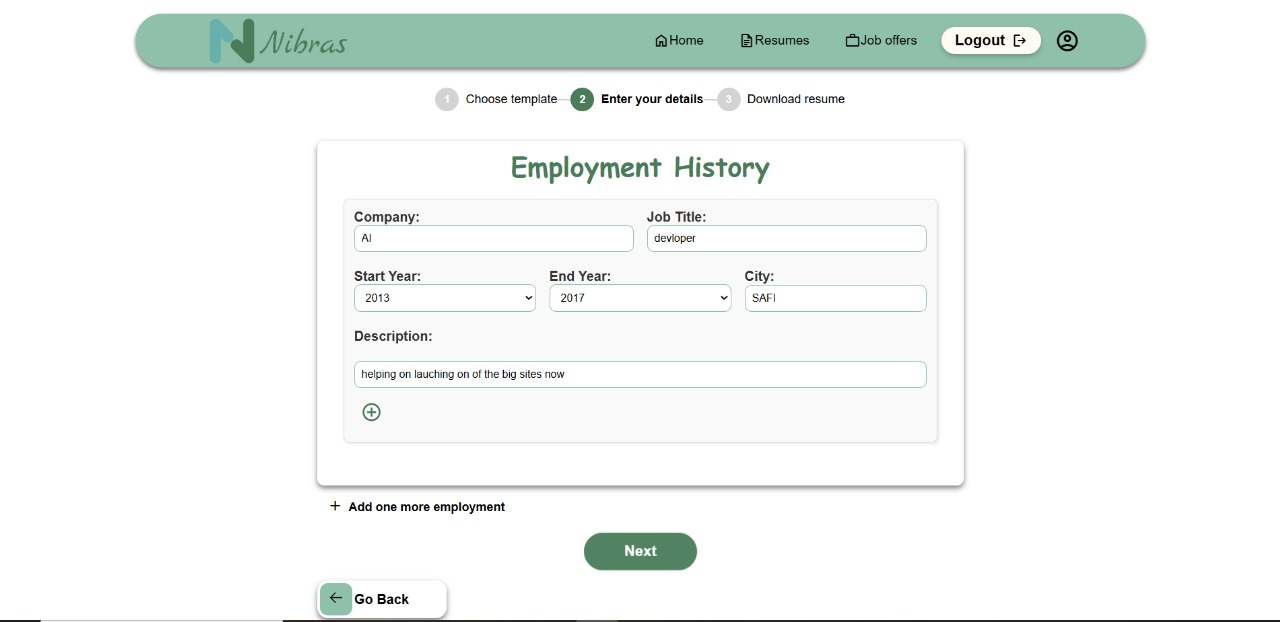
\includegraphics[width=1.2\linewidth]{./imgs/screens/empForm.jpg}
    \caption{Formulaire pour les informations des experiences requises}
\end{figure} 

\begin{figure}[h]
    \centering
    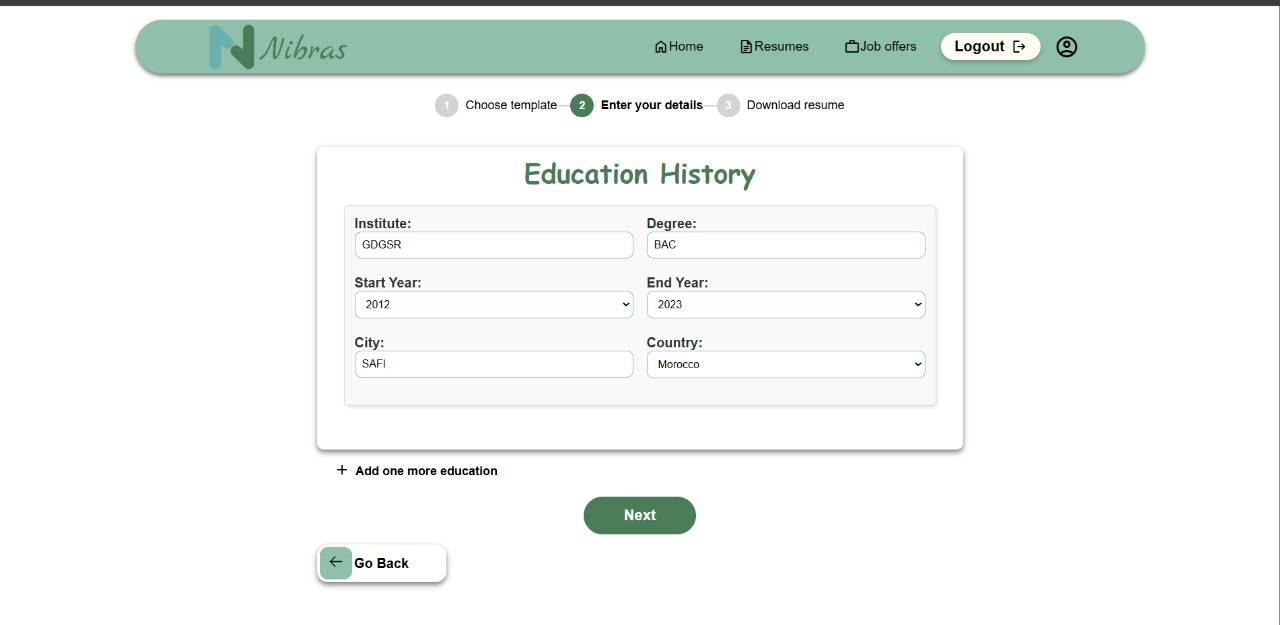
\includegraphics[width=1.2\linewidth]{./imgs/screens/eduForm.jpg}
    \caption{Formulaire pour les informations d'éducation}
\end{figure} 

\begin{figure}[h]
    \centering
    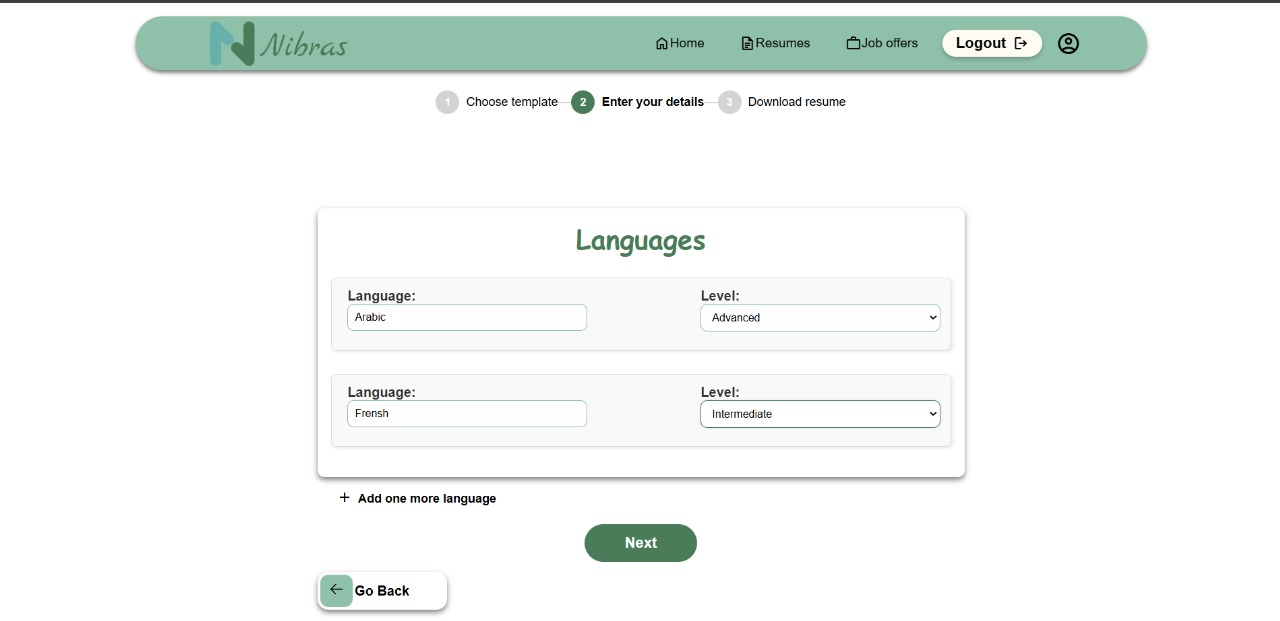
\includegraphics[width=1.2\linewidth]{./imgs/screens/langForm.jpg}
    \caption{Formulaire pour les informations des langues}
\end{figure}

\begin{figure}[h]
    \centering
    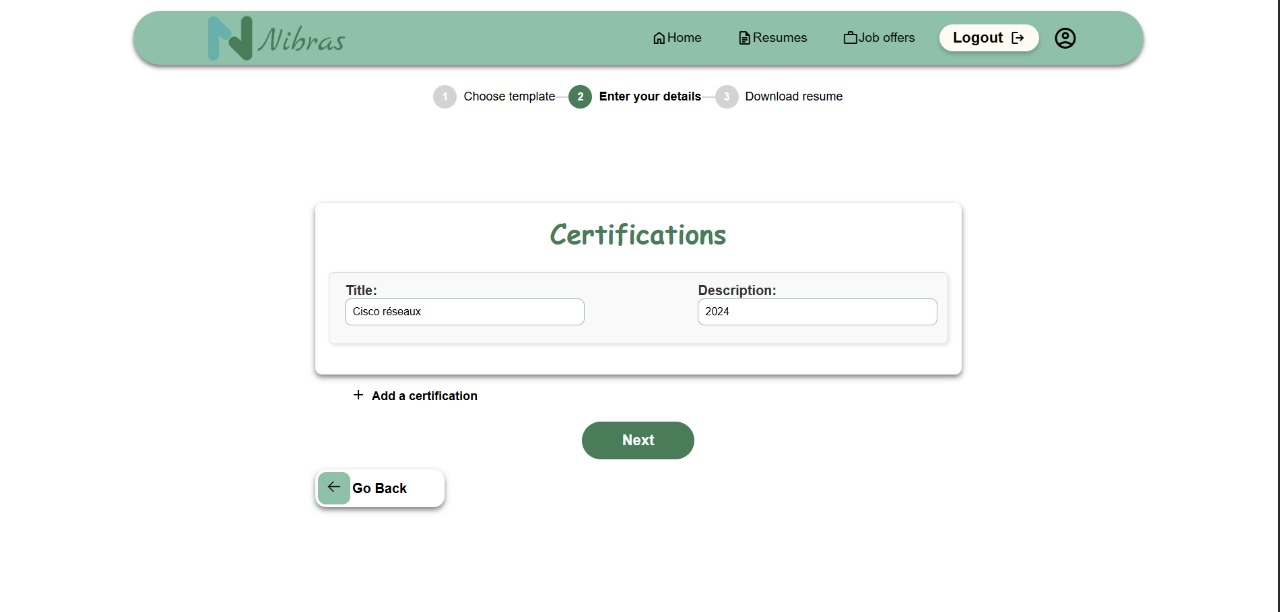
\includegraphics[width=1.2\linewidth]{./imgs/screens/certifForm.jpg}
    \caption{Formulaire pour les informations des certtifications}
\end{figure} 

\begin{figure}[h]
    \centering
    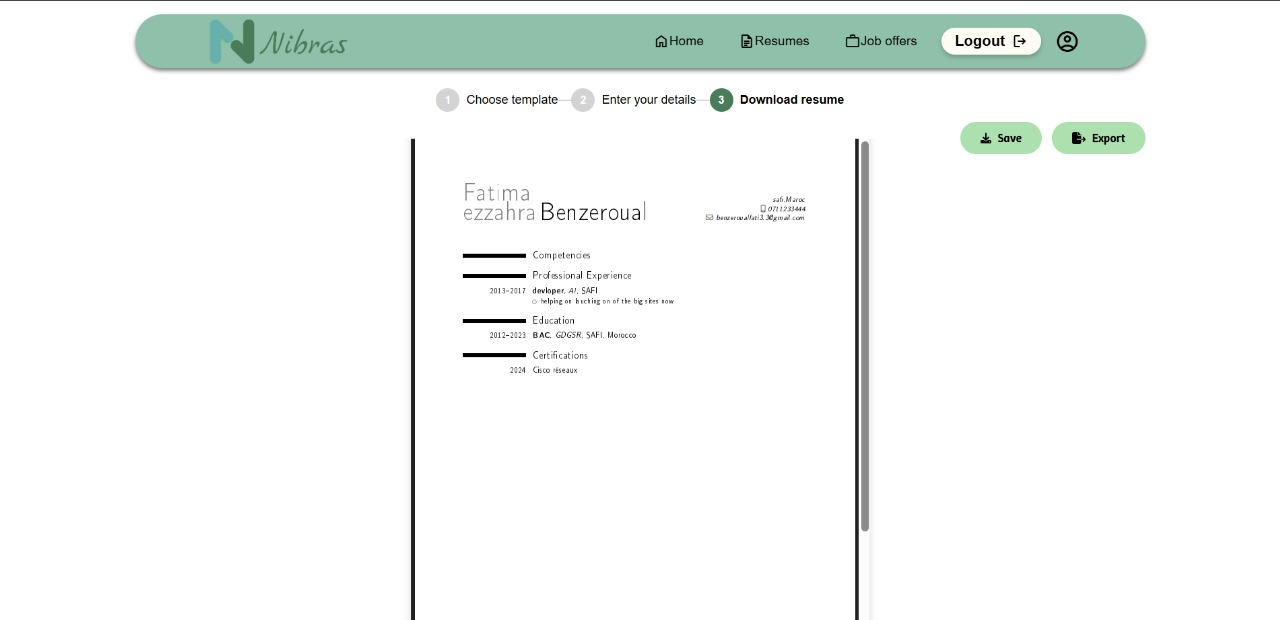
\includegraphics[width=1.2\linewidth]{./imgs/screens/previewResume.jpg}
    \caption{Apercu du CV crée avec boutton de sauvegarde et téléchargement}
\end{figure} 

\clearpage
\subsubsection{Creation d'offre d'emploi}
\begin{figure}[h]
    \centering
    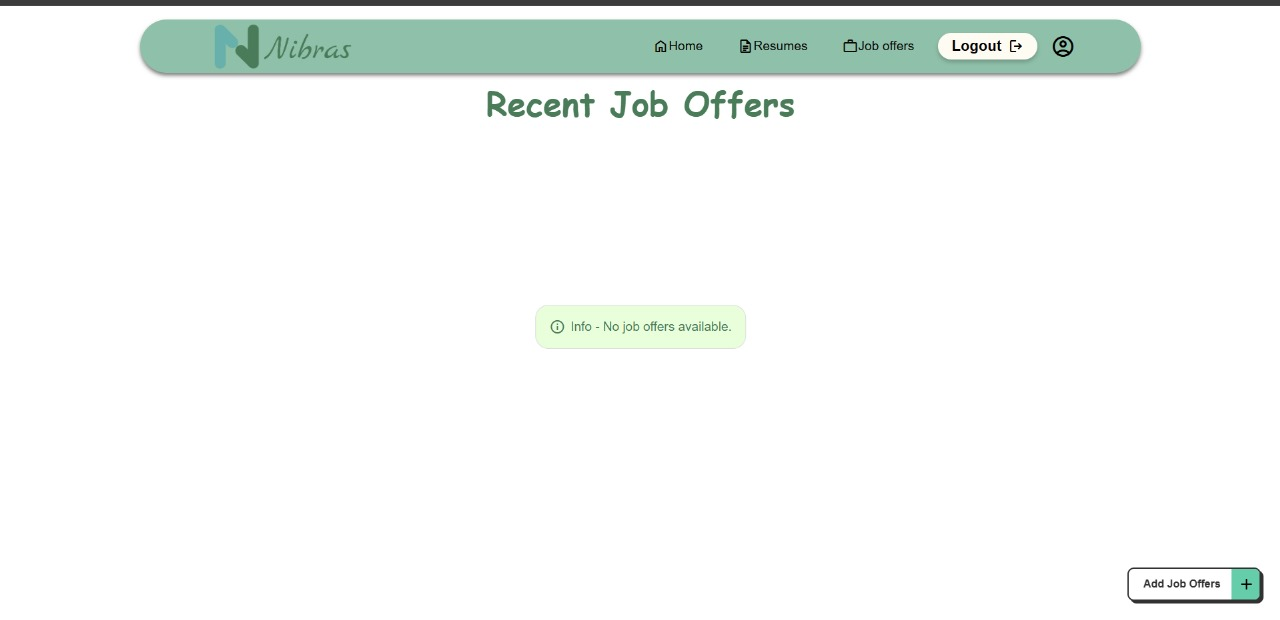
\includegraphics[width=1.2\linewidth]{./imgs/screens/emptyJobOffer.jpg}
    \caption{Interface de publication d'offre d'emploi (vide)}
\end{figure} 

\begin{figure}[h]
    \centering
    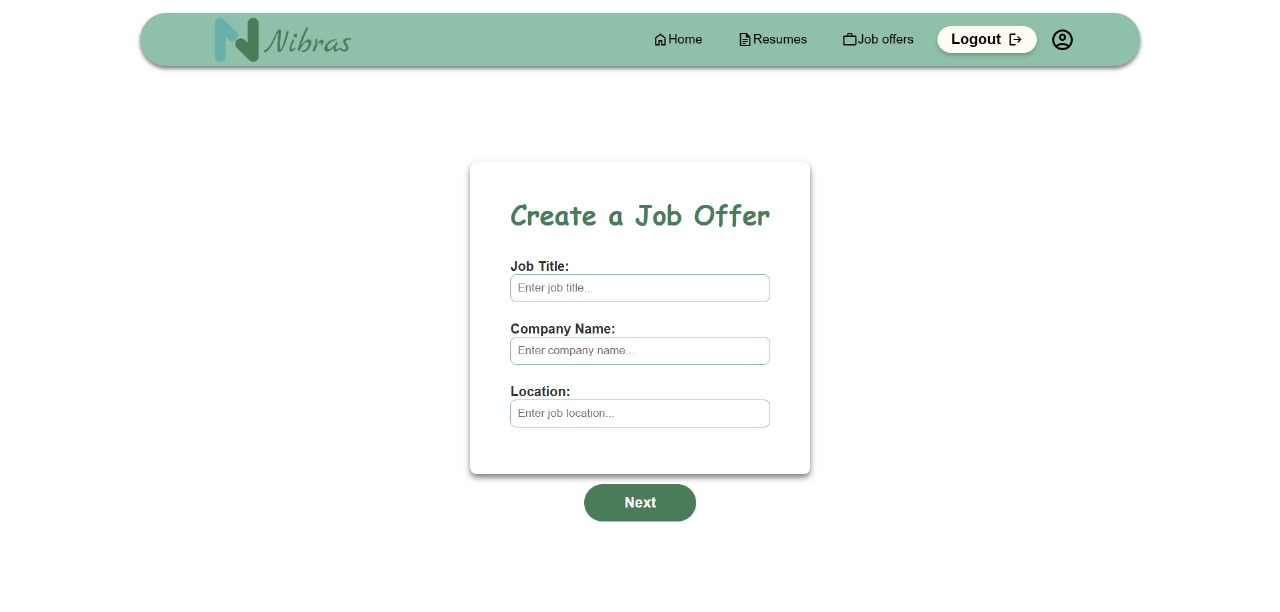
\includegraphics[width=1.2\linewidth]{./imgs/screens/createJobOffer.jpg}
    \caption{Ajouter un nouvelle Offre d'emploi}
\end{figure} 
\vspace{2cm}

\begin{figure}[h]
    \centering
    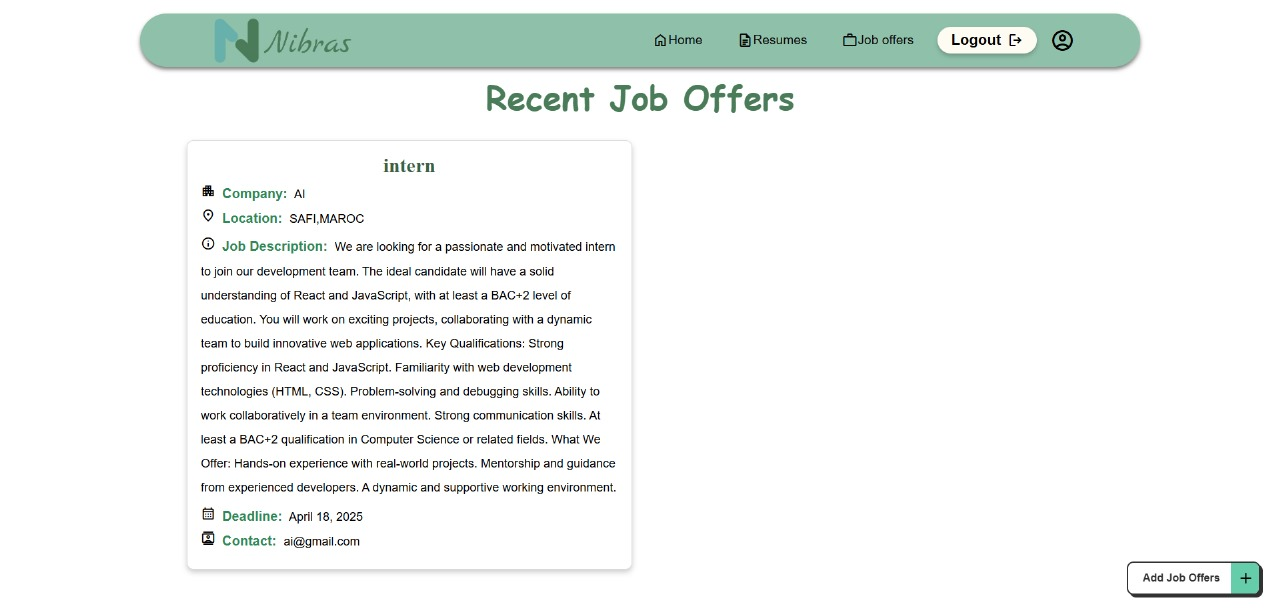
\includegraphics[width=1.2\linewidth]{./imgs/screens/jobOfferList.jpg}
    \caption{Interface de publication d'offre d'emploi (après création d'offre)}
\end{figure} 

\clearpage
\subsubsection{Profile}
\begin{figure}[h]
    \centering
    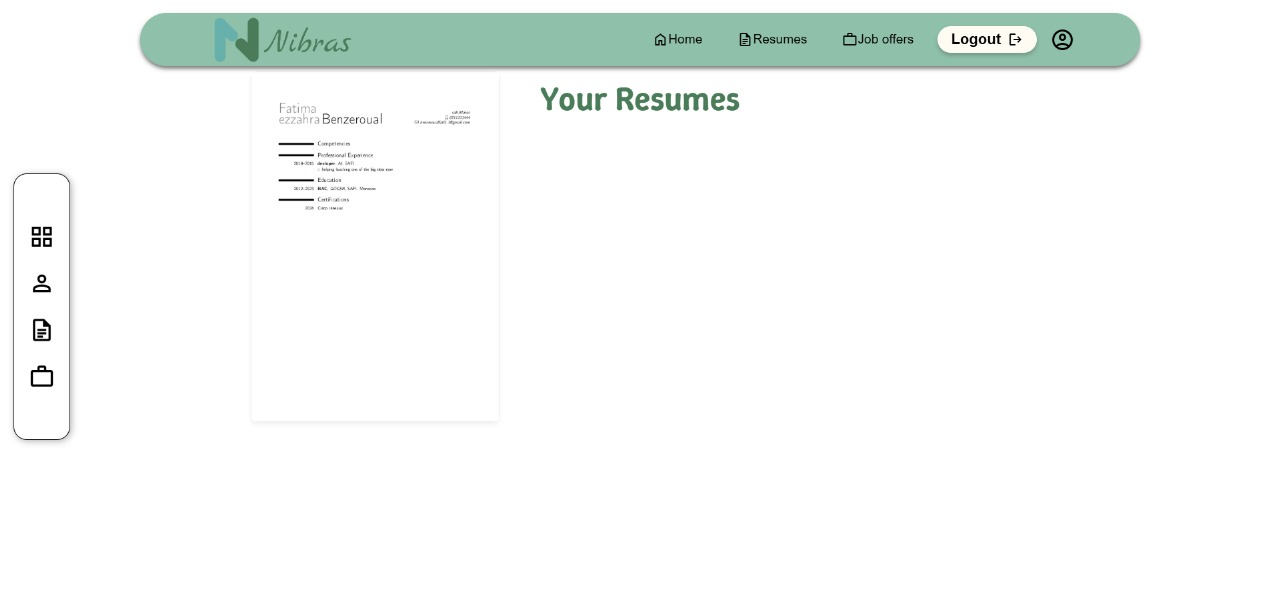
\includegraphics[width=1.2\linewidth]{./imgs/screens/userResumes.jpg}
    \caption{Les cv crées par l'utilisateur connectés} 
\end{figure} 

\begin{figure}[h]
    \centering
    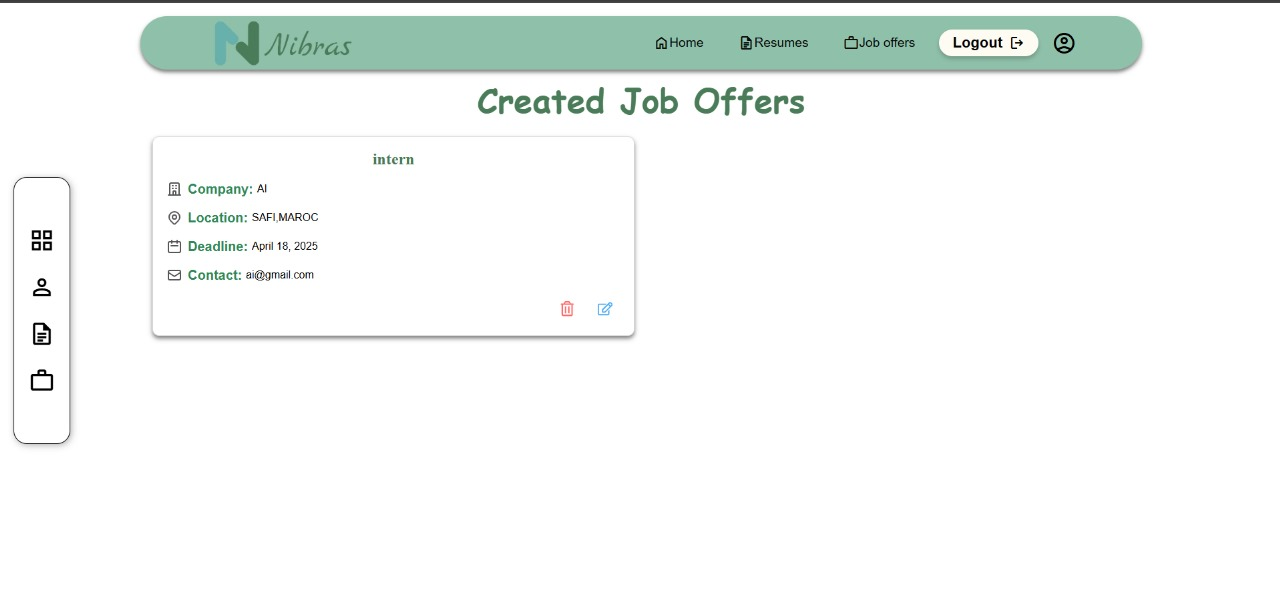
\includegraphics[width=1.2\linewidth]{./imgs/screens/userJobOffers.jpg}
    \caption{Les offres d'emploi crées par l'utilisateur connectés} 
\end{figure} 

\begin{figure}[h]
    \centering
    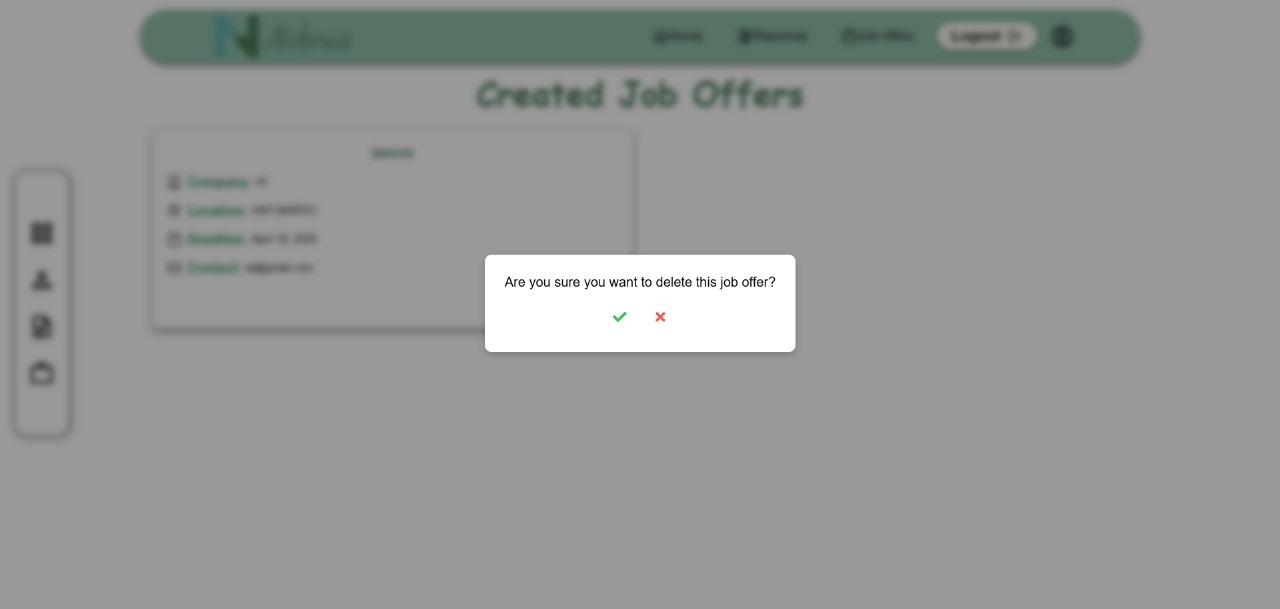
\includegraphics[width=1.2\linewidth]{./imgs/screens/userResumesDelete.jpg}
    \caption{Supprimer un offre d'emploi déjà crée} 
\end{figure} 

\begin{figure}[h]
    \centering
    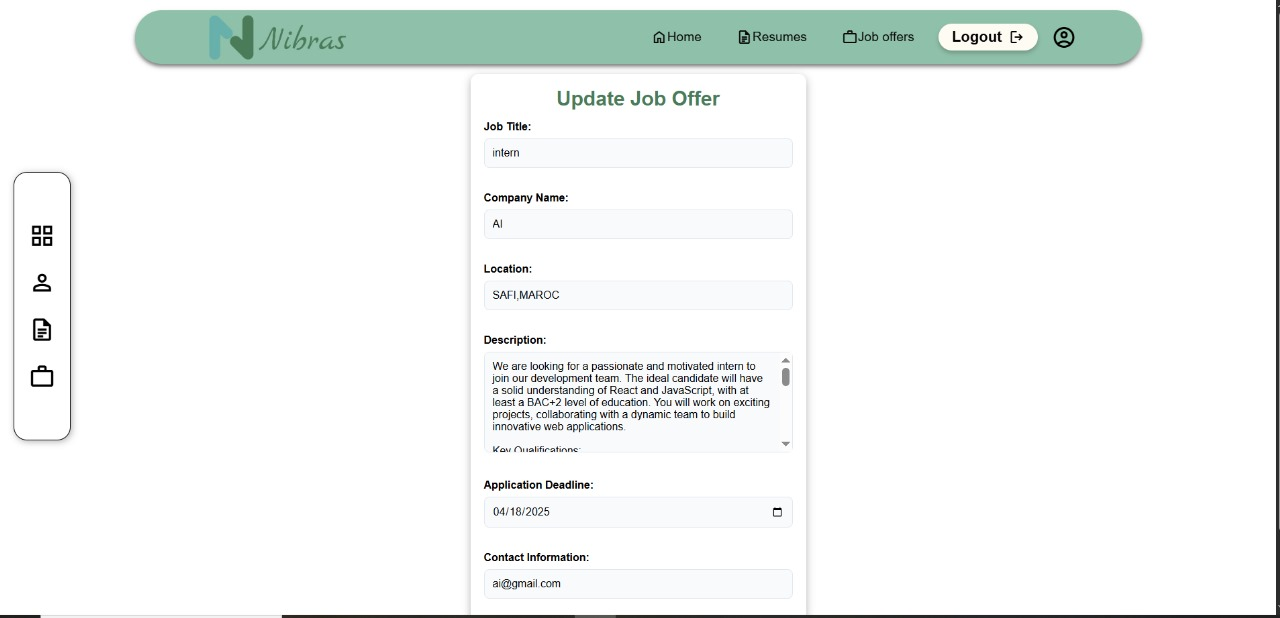
\includegraphics[width=1.2\linewidth]{./imgs/screens/userResumesUpdate.jpg}
    \caption{Modifier un offre d'emploi déjà crée} 
\end{figure} 

\begin{figure}[h]
    \centering
    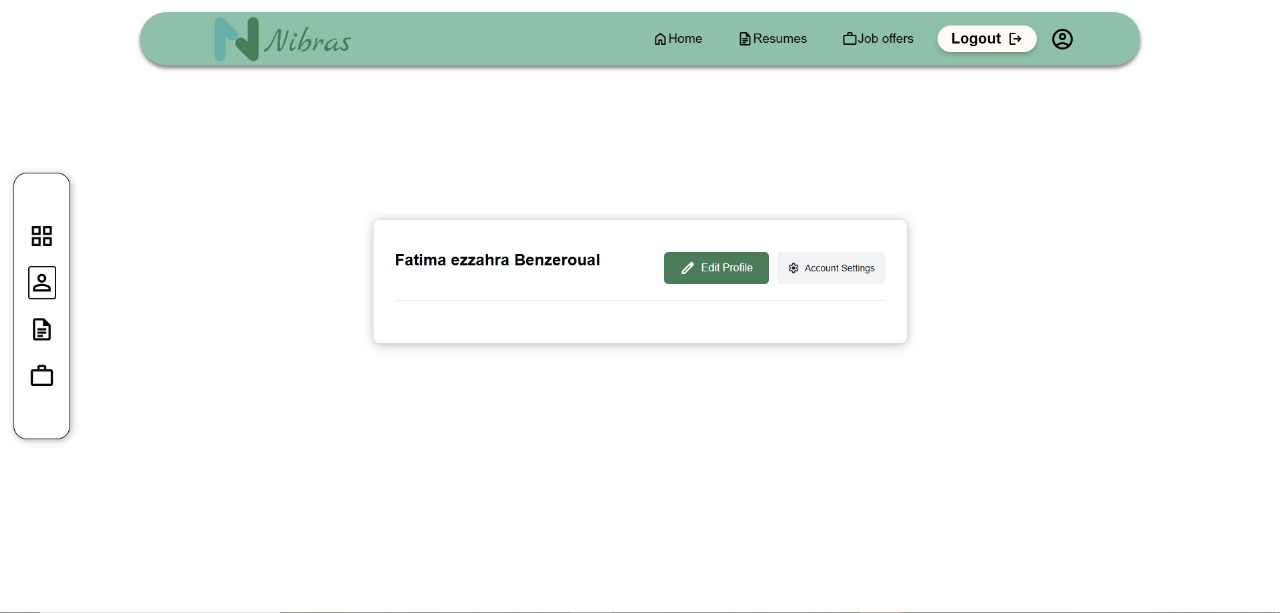
\includegraphics[width=1.2\linewidth]{./imgs/screens/profileActions.jpg}
    \caption{Actions de profile} 
\end{figure} 

\begin{figure}[h]
    \centering
    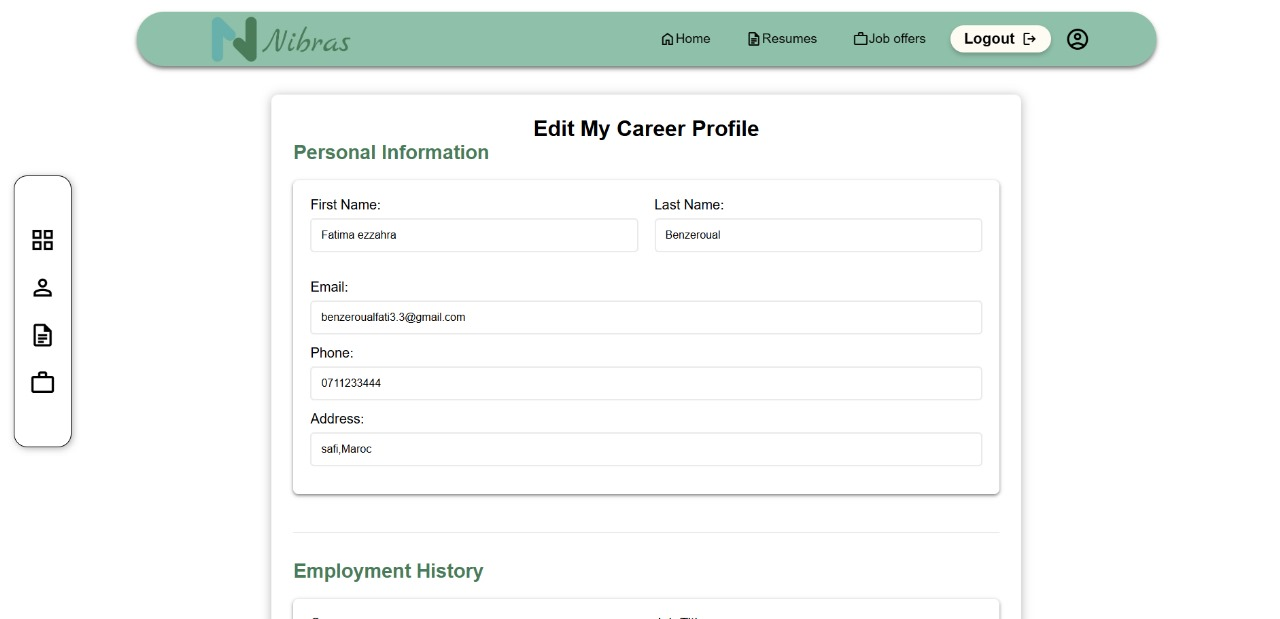
\includegraphics[width=1.2\linewidth]{./imgs/screens/userInfoEdit.jpg}
    \caption{Modifier/remplir les informations de l'utilisateur} 
\end{figure} 

\begin{figure}[h]
    \centering
    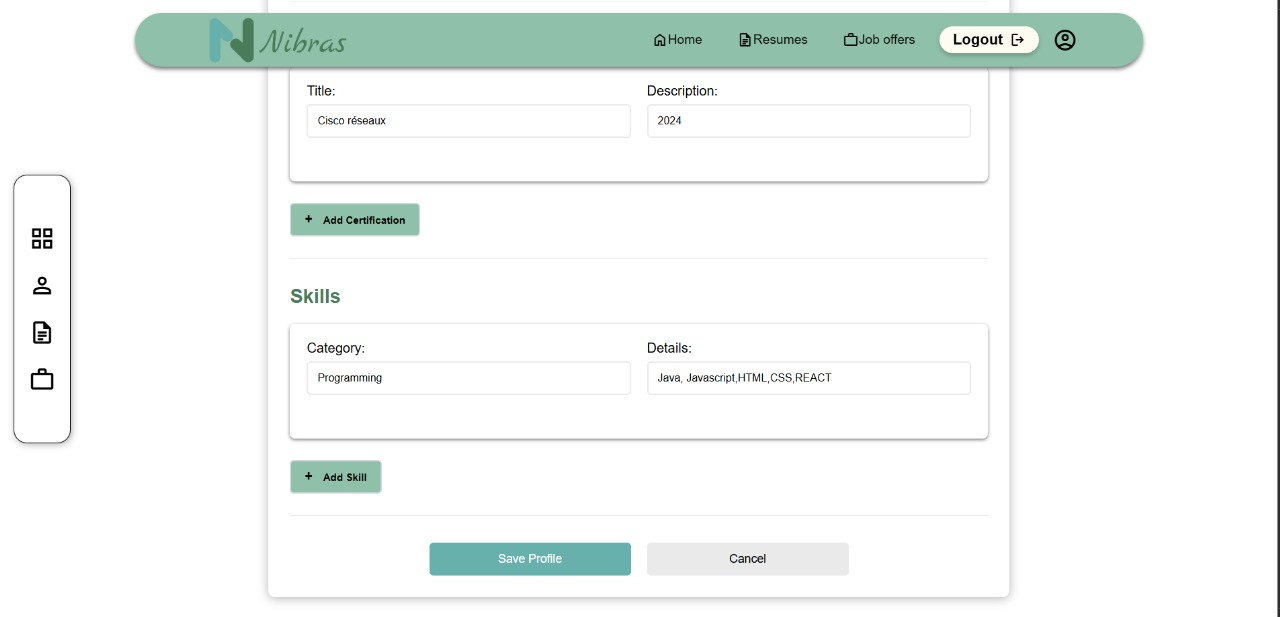
\includegraphics[width=1.2\linewidth]{./imgs/screens/userInfoEdit2.jpg}
    \caption{Modifier/remplir les informations de l'utilisateur (suite)} 
\end{figure} 

\begin{figure}[h]
    \centering
    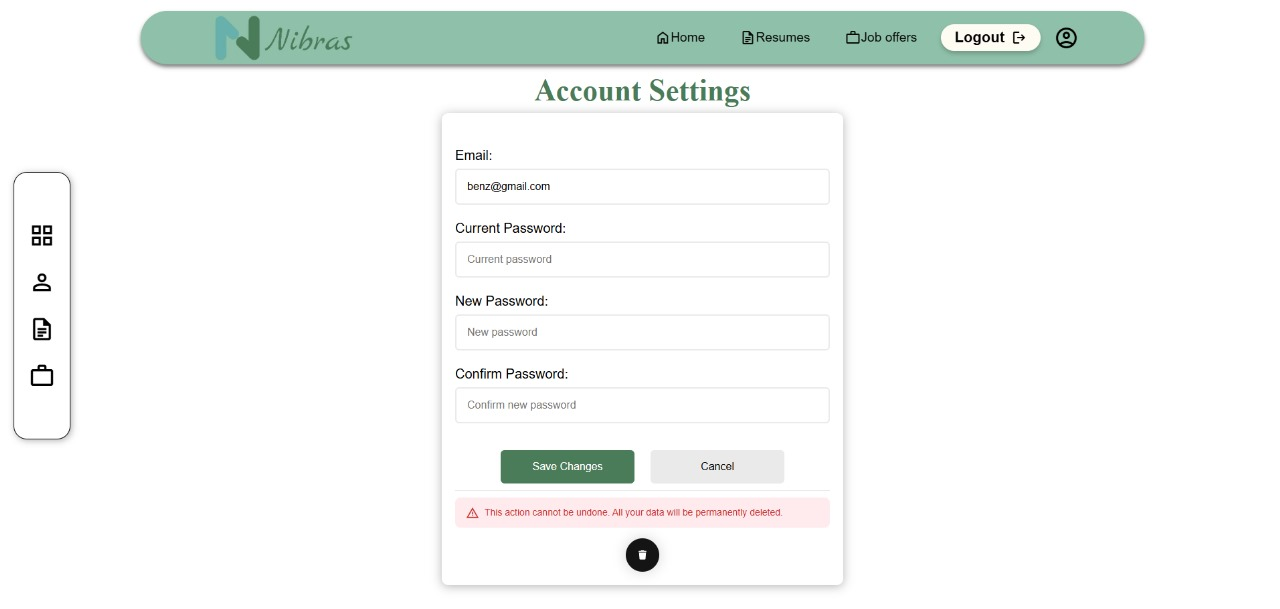
\includegraphics[width=1.2\linewidth]{./imgs/screens/userAuthEdit.jpg}
    \caption{Modifier les informations d'authentification de l'utilisateur} 
\end{figure} 
\begin{figure}[h]
    \centering
    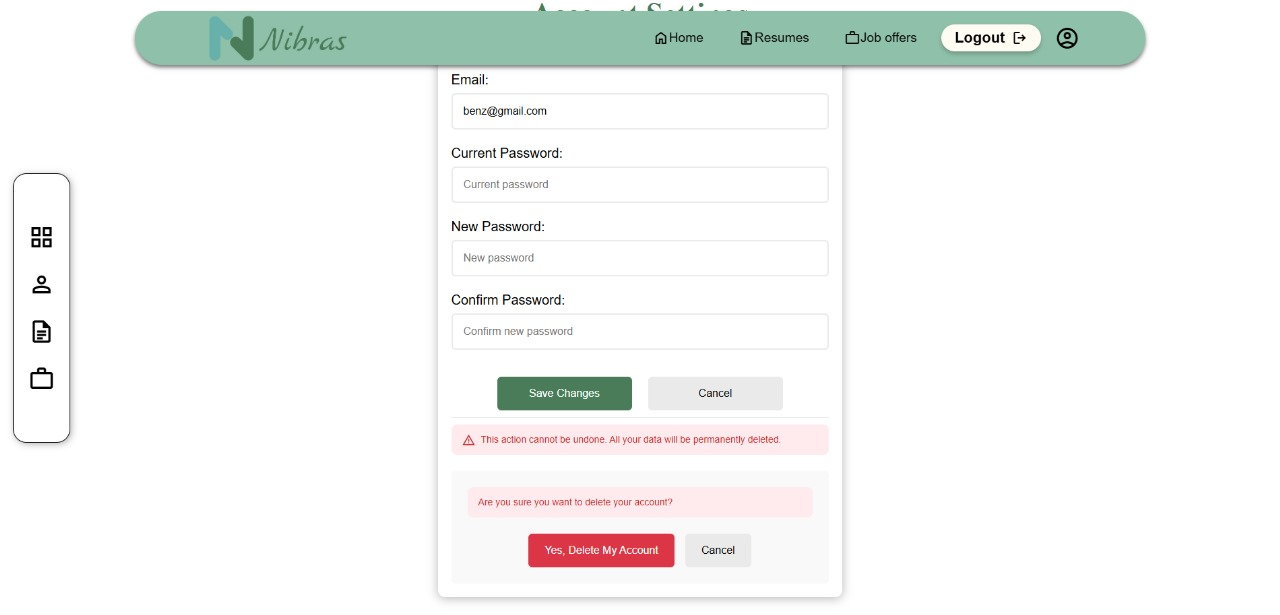
\includegraphics[width=1.2\linewidth]{./imgs/screens/userAuthDelete.jpg}
    \caption{Supprimer le compte de l'utilisateur} 
\end{figure} 
\begin{figure}[h]
    \centering
    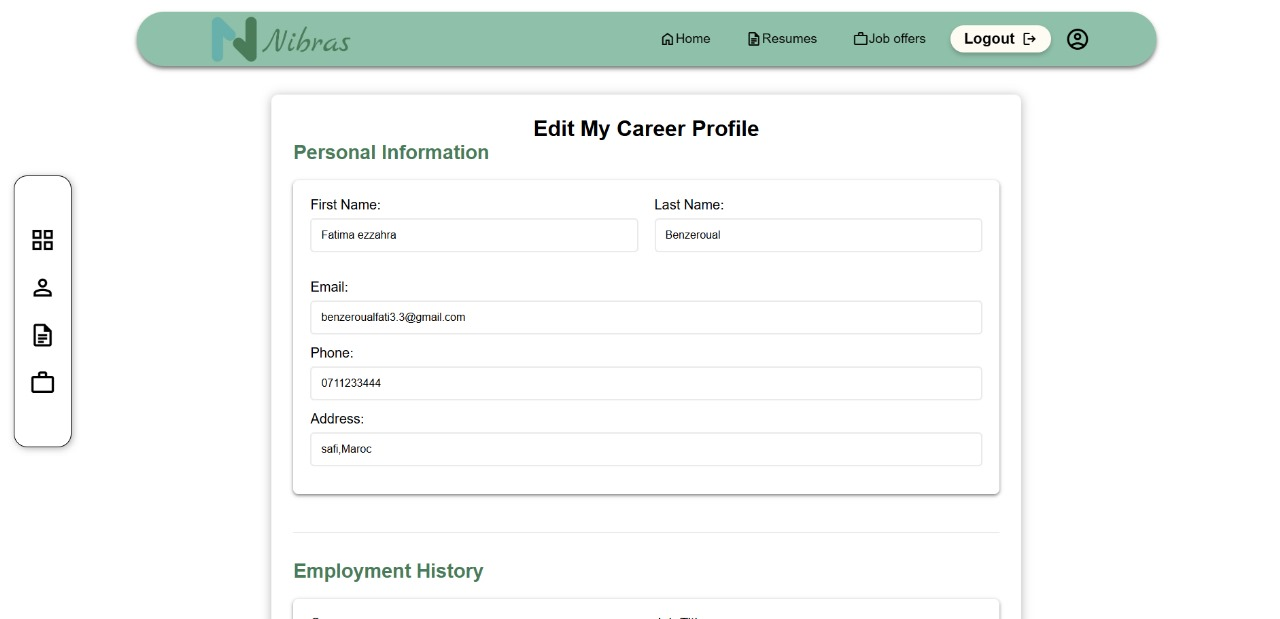
\includegraphics[width=1.2\linewidth]{./imgs/screens/userInfoEdit.jpg}
    \caption{Modifier/remplir les informations de l'utilisateur} 
\end{figure} 


%\subsection{Espace administrateurs}
%\subsubsection{Gestion des templates}
%\subsubsection{statistiques}


\section{Conclusion}
Cette implémentation a validé la faisabilité technique de la plateforme tout en identifiant des axes d'optimisation, notamment pour la génération de documents et l'expérience utilisateur. L'architecture retenue (MERN + LaTeX) s'est révélée adaptée aux besoins du projet.



\chapter{Conclusion}
\clearpage


\vspace*{\fill} % Vertical centering

Ce projet a permis de développer une plateforme fonctionnelle de création de CV en LaTeX, combinant avec succès les technologies web modernes (React, Express, MongoDB) et les capacités typographiques avancées de LaTeX. L'application répond aux objectifs initiaux en offrant une interface intuitive pour la génération de documents professionnels, tout en intégrant un système de gestion des offres d'emploi et un panneau d'administration.

\vspace{1cm} % Additional vertical space

Les principaux défis techniques, notamment la compilation serveur de PDF et la gestion des données semi-structurées, ont été résolus grâce à une architecture modulaire. Bien que certaines limitations persistent, comme les temps de génération des documents ou les possibilités limitées de personnalisation avancée, la solution ouvre des perspectives intéressantes pour l'automatisation de processus RH.

\vspace{1cm} % Additional vertical space

Ce travail démontre qu'il est possible de moderniser des workflows documentaires traditionnels tout en préservant leurs exigences de qualité, et pourrait être étendu à d'autres types de documents professionnels à l'avenir.

\vspace*{\fill} % Vertical centering

\section*{Références}
\begin{itemize}
    \item https://uiverse.io/
    \item https://fonts.google.com/
    \item https://fontawesome.com/
    \item https://github.com/Fatim-ezzahrae/PFEProject.git
    \item https://chat.deepseek.com/
    \item https://chatgpt.com/
    \item https://www.logoai.com/
    \item https://coolors.co/
\end{itemize}


\addcontentsline{toc}{section}{Références}  % Add Références to TOC


\end{document}